\clearpage
\section{Durchführung und Auswertung}
%
\subsection{Warnhinweise}\label{sec:warnhinweise}
%
\begin{minipage}[c]{.15\linewidth}
	
\includegraphics[width=1.5cm]{img/toxic}
\end{minipage}
\begin{minipage}[t]{.85\linewidth}
	Essen und Trinken ist im Labor untersagt.
\end{minipage}\vspace{1em}\\ 
\begin{minipage}[c]{.15\linewidth}
	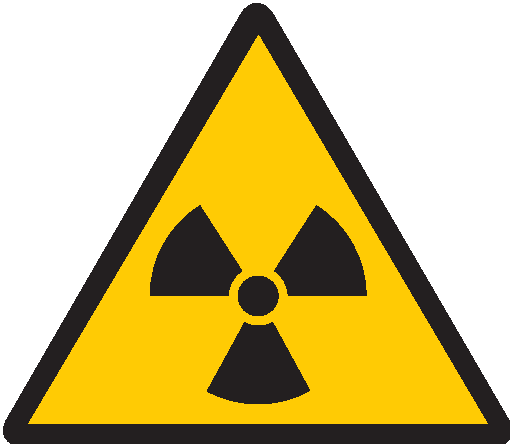
\includegraphics[width=1.5cm]{img/radioactive}
\end{minipage}
\begin{minipage}[t]{.85\linewidth}
	Die verwendete Strahlungsquelle sendet radioaktive Alphastrahlung aus. Sie ist schwach versiegelt und teilweise offen. Der Strahlenschutz sieht für solche Quellen besondere Sicherheitsmaßnahmen vor. Deshalb wurde das Präparat dauerhaft in der Apparatur installiert, sodass kein radioaktives Material aus der Apparatur in den Raum gelangen kann und kein Kontakt mit der Quelle möglich ist. Die Messapparatur darf deshalb auf keinen Fall geöffnet werden. Das Belüftungsventil soll so kurz wie möglich geöffnet bleiben.
\end{minipage}\vspace{1em}\\ 
\begin{minipage}[c]{.15\linewidth}
	
\includegraphics[width=1.5cm]{img/electric}
\end{minipage}
\begin{minipage}[t]{.85\linewidth}
	Die maximale Spannung am Halbleiterdetektor beträgt $200$ Volt. Die Spannung immer langsam verändern. Überschreiten der Spannung kann zur Zerstörung des Detektors führen.
	\\ \\
	Änderungen an der Verkabelung nur bei abgeschalteter Spannungsversorgung.
	\\ \\
	Der Detektor ist extrem lichtempfindlich, der Betrieb mit angelegter Hochspannung außerhalb der geschlossenen Vakuumkammer würde ihn zerstören.
\end{minipage}\vspace{1em}\\ 
\begin{minipage}[c]{.15\linewidth}
	
\includegraphics[width=1.5cm]{img/attention}
\end{minipage}
\begin{minipage}[t]{.85\linewidth}
	Be- und Entlüftungsventil des Vakuumkolbens nicht gleichzeitig öffnen.
	\\ \\
	Vor dem Be- oder Entlüften die Hochspannung abschalten. 
\end{minipage}\vspace{1em}\\ 
%
\clearpage
%
\subsection{Vorbereitungen}
Gehen Sie diese Checkliste gemeinsam mit dem/der Betreuer:in durch:
\begin{enumerate}
	\item Verkabelung kontrollieren (vgl. Abb. \ref{fig:verkabelung}).
	\item Sicherstellen, dass das Spannungsversorgungsgerät auf $0$ V eingestellt ist.
	\item Quelle auf kleinstmöglichen Abstand zum Detektor einstellen \\$r_{rel} = 0$ mm.
	\item Vakuumkammer evakuieren.
	\item Ortec-Crate einschalten.
	\item MCA3 Software auf dem PC starten.
\end{enumerate}

%
\subsection{Aufgabe 1: Sättigungsspannung}
Ziel der ersten Aufgabe ist die Bestimmung der Sättigungsspannung des Halbleiterdetektors. Die Messung erfolgt im Vakuum bei kleinstmöglichem Abstand $r_{rel} = 0$ mm.
\begin{enumerate}[label=\textbf{\alph*)}]
	\item Zeichnen Sie bei Detektorspannung $U_A = 0$ V ein Histogramm mit mindestens 8000 Counts auf. Bestimmen Sie 
		\begin{itemize}[nosep]
		\item die Peak-Position $\mu\ [\text{ADC Channels}]$,
		\item die Halbwertsbreite \textit{FWHM} [ADC Channels]
		\item und die Zählrate $Z$ [1/s]
	\end{itemize}
	des Plutonium-Peaks mithilfe eines Gauß-Fits in der Software.
	\item Wiederholen Sie a) für die Spannungen $U_A = 8, 15, 20, 25, 30, 40, 70, 100$ V
	\item Stellen Sie die Peak-Position $\mu$, die Zählrate $Z$ und die prozentuale Auflösung
		\begin{equation}
			d_E = \frac{\textit{FWHM}}{\mu} \cdot 100 \qquad [\%]
		\end{equation}
		in Abhängigkeit von $U_A$ grafisch dar.
	\item Bestimmen Sie ungefähr die Sättigungsspannung $U_{\text{sat.}}$ des Detektors anhand der Kurvenverläufe. Wählen Sie eine Spannung $U_{\text{Det.}}$ für Ihre folgenden Messungen. Erklären Sie Ihre Auswahl und die Bedeutung der Sättigungsspannung für die Benutzung des Halbleiterdetektors zum Energienachweis.
\end{enumerate}

\subsection{Aufgabe 2: Kalibrierung und Nullabstand}
Nun wird eine Energiekalibrierung des Multi-Channel-Analysators durchgeführt und der Nullabstand $r_0$ zwischen Detektor und Quelle bestimmt. Die Messungen finden im Vakuum statt.

\begin{enumerate}[label=\textbf{\alph*)}]
	\item Stellen Sie die in Aufgabe 1 ermittelte Spannung $U_{\text{Det.}}$ an der Spannungsversorgung ein.
	\item Zeichnen Sie ein Referenzspektrum mit mindestens 12000 Counts bei $r_{rel} = 0$ mm auf. Speichern Sie einen Screenshot des Referenzspektrums für Ihr Protokoll.
		\\ \textit{Optional:} Speichern Sie das Histogramm als \verb|.txt| Datei ab. Dies ermöglicht die Wiederholung der Kalibrierung zu Hause. 
	\item Kalibrieren Sie den Multi-Channel-Analyzer in der Software. \\Bestimmen Sie dazu die Position der drei Hauptmaxima im Histogramm per Gauß-Fit und verwenden Sie die passenden Austrittsenergien aus Abbildung~\ref{fig:schemata}.
	
	Führen Sie die Gauß-Fits erneut durch, um die kalibrierten Werte für Positionen [keV] und Halbwertsbreiten [keV] sowie die Zählraten [1/s] zu erhalten.
	\item Zeichnen Sie bei den relativen Abständen $r_{rel} = 5, 10, 15, 20, 30$ mm jeweils mindestens 3000 Counts auf und bestimmen Sie auch hier per Gauß-Fit die kalibrierten Positionen, Halbwertsbreiten und Zählraten der drei Hauptmaxima.
	\item \textit{Am Versuchstag:} Stellen Sie die Zählrate in Abhängigkeit des relativen Abstandes für Plutonium grafisch dar.
	
	\textit{Im Protokoll:} Stellen Sie die Energie, die prozentuale Detektorauflösung und die Zählrate  jeweils in Abhängigkeit des relativen Abstandes für jedes der drei Isotope grafisch dar.
	\item Bestimmen Sie den Nullabstand $r_0$ zwischen Probe und Detektor, um bei den weiteren Messungen den effektiven Abstand $r_{eff} = r_0 + r_{rel}$ verwenden zu können. Überlegen Sie dazu, wie das Abstandsgesetz
	\begin{equation}
		Z \propto \frac{1}{r^2_{eff}}
	\end{equation}
	umgeformt und geschickt grafisch dargestellt werden kann, um den Nullabstand direkt vom y-Achsenabschnitt ablesen zu können. $Z$ ist hier die Zählrate $[1/s]$. Errechnen Sie das gemittelte Ergebnis aus den Messungen aller drei Isotope und stellen alle Werte in einer Tabelle dar.

    \textit{Anmerkung}: Betrachten Sie die Fehlerbalken und entscheiden Sie, ob Sie den einfachen oder den gewichteten Mittelwert verwenden, um das Endergebnis zu erhalten. Siehe hierzu Gleichung~\eqref{eq:weighted_mean} auf Seite~\pageref{eq:weighted_mean} im Anhang.
	

\end{enumerate}

\subsection{Aufgabe 3: Reichweite in Luft}
Im letzten Teil des Versuches wird der differenzielle Energieverlust der Alphastrahlung in Luft bestimmt.

\begin{enumerate}[label=\textbf{\alph*)}]
	\item Schließen Sie das Entlüftungsventil der Vakuumkammer. Öffnen Sie danach langsam das Belüftungsventil, bis der Atmosphärendruck in der Kammer hergestellt ist. Schließen Sie dann das Belüftungsventil wieder.
	\item Bestimmen Sie bei $r_{rel} = 0, 4, 8, 20, 24, 28, 32, 36, \dots$ mm mittels Gauß-Fit
	\begin{itemize}[nosep]
		\item die kalibrierte Peakposition $\mu\ [\text{keV}]$,
		\item die kalibrierte Halbwertsbreite \textit{FWHM} [keV]
		\item und die Zählrate $Z$ [1/s]
	\end{itemize}
	für die Hauptmaxima der drei Isotope. Erhöhen Sie den relativen Abstand weiter um je $4$ mm, bis das Plutoniumsignal bei $r_{max}$ verschwindet. Führen Sie dann noch drei zusätzliche Messungen bei $r_{rel} = r_{max} - 2, r_{max} - 6, r_{max} - 10$ mm durch. Zeichnen Sie für jede Messung mindestens 2000 Counts auf.
	\item \textit{Am Versuchstag:} Stellen Sie die $\alpha$-Energie $E\, \widehat{=}\, \mu$ abhängig vom effektiven Abstand für Plutonium grafisch dar.
	
	\textit{Im Protokoll:} Stellen Sie für alle drei Isotope die $\alpha$-Energie $E\, \widehat{=}\, \mu$, die prozentuale Auflösung und die Zählrate jeweils in Abhängigkeit vom effektiven Abstand grafisch dar.
	\item Bestimmen Sie näherungsweise -- durch Extrapolation mit dem Auge -- die Reichweite der $\alpha$-Teilchen ($R$) und ihre Austrittsenergie ($E_0$) anhand des Graphen, der effektiven Abstand gegen Energie zeigt. Wodurch wird die Unsicherheit der Ergebnisse am stärksten beeinflusst?
	
	Vergleichen Sie in einer Tabelle die Ergebnisse mit den Literaturwerten. Verwenden Sie dazu die angegebenen Austrittsenergien und das empirische Reichweitengesetz von Geiger, welches die Reichweite $R$ [mm] abhängig von der Austrittsenergie $E_0$ [MeV] der $\alpha$-Teilchen angibt:
	\begin{equation}\label{eq:geigerreachlaw}
		R = 3.1 \cdot \left(E_0\right)^{3/2}
	\end{equation}
	\textit{Optional:} Wenn Gleichung~\eqref{eq:geigerreachlaw} entsprechend umgeformt und angepasst wird, eignet sie sich als Fit-Funktion für die Daten. Damit können Reichweite und Austrittsenergie genauer als mit dem Auge bestimmt werden.
	\item \textit{Am Versuchstag:} Stellen Sie den differenziellen Energieverlust in Abhängigkeit des effektiven Abstands für Plutonium dar $\left( \Delta E/ \Delta x \ \text{vs.}\ r_{eff} \right)$.
	
	\textit{Im Protokoll:} Fügen Sie die Bragg-Kurven der anderen beiden Isotope hinzu. Schätzen Sie den Höchstwert des Energieverlusts und den Energieverlust in der Nähe der Probe. Vergleichen Sie die drei Kurven miteinander.
	\item Schätzen Sie die unterschiedlichen Beiträge ab, die in die Energieauflösung einfließen. Betrachten Sie die Detektorauflösung aus der Vakuum"= und der Luft"=Messung. Diskutieren Sie hierbei die Bedeutung des elektronischen Rauschens, der statistischen Schwankungen in der Anzahl der Elektronen"=Loch"=Paare (Fanofaktor), sowie die endliche Dicke des Strahler-Präparats und das Energiestraggeling.
\end{enumerate}
%
%





